% Signal Hierarchy Petri Nets - Drug Discovery Application
% PLOS Computational Biology Format
% Version: January 25, 2026

\documentclass[10pt,letterpaper]{article}
\usepackage[top=0.85in,left=2.75in,footskip=0.75in]{geometry}

% amsmath and amssymb packages, useful for mathematical formulas and symbols
\usepackage{amsmath,amssymb,amsfonts,amsthm}

% Use adjustwidth environment to exceed column width (see example table in text)
\usepackage{changepage}

% textcomp package and marvosym package for additional characters
\usepackage{textcomp,marvosym}

% cite package, to clean up citations in the main text. Do not remove.
\usepackage{cite}

% Use nameref to cite supporting information files
\usepackage{nameref,hyperref}

% line numbers
\usepackage[right]{lineno}

% ligatures disabled
\usepackage[nopatch=eqnum]{microtype}
\DisableLigatures[f]{encoding = *, family = * }

% color can be used to apply background shading to table cells only
\usepackage[table]{xcolor}

% array package for better arrays (eg matrices) in maths
\usepackage{array}

% verbatim environment for code and preformatted text
\usepackage{verbatim}

% booktabs for professional tables
\usepackage{booktabs}

% multirow for complex tables
\usepackage{multirow}

% float package for H placement specifier
\usepackage{float}

% siunitx for SI units
\usepackage{siunitx}
\DeclareSIUnit\Molar{M}
\DeclareSIUnit\molar{M}

% graphicx for including figures
\usepackage{graphicx}

% subcaption for subfigures
\usepackage{subcaption}

% mhchem for chemical formulas
\usepackage[version=3]{mhchem}

% Custom commands
\newcommand{\etal}{\textit{et al.}}

% Remove paragraph indentation
\setlength{\parindent}{0pt}
\setlength{\parskip}{6pt}

\begin{document}
\vspace*{0.2in}

% Title must be 250 characters or less
\begin{flushleft}
{\Large
\textbf{Signal Hierarchy Petri Nets for Energy-Dependent Biochemical Systems: High-Throughput \textit{In Silico} Analysis of Macrocyclic Peptide Transport and Stability}
}
\newline
% Insert author names, affiliations and corresponding author email
\\
Eug\^enio Sim\~ao$^{1,*}$
\\
\bigskip
\textbf{1} Department of Computer Science, Universidade Federal de Santa Catarina (UFSC), Ararangu\'a, Santa Catarina, 88906-072, Brazil
\\
\bigskip

% Use the asterisk to denote corresponding authorship and provide email address
* eugenio.simao@ufsc.br

\end{flushleft}

% Please keep the abstract below 300 words
\section*{Abstract}
Modeling energy-dependent biochemical systems requires formalisms that capture how metabolic state hierarchically controls pathway selection. Classical Petri net approaches treat ATP as a passive metabolite rather than an active regulatory signal, lacking formal semantics for hierarchical pathway preemption based on energy availability. We introduce Signal Hierarchy Petri Nets, a computational formalism organizing biochemical pathways into energy-dependent layers enabling ATP to function simultaneously as metabolite (consumed in reactions) and regulatory signal (controlling layer activation). The formalism provides layered pathway architecture with explicit ATP dependencies, signal place partitioning distinguishing regulatory signals from metabolic species, hierarchical firing rules enabling upper layers to preempt lower layers when energy permits, and dual ATP semantics capturing both mass transfer and regulatory control.

We demonstrate the formalism's predictive capability through systematic \textit{in silico} screening of macrocyclic peptide transport and stability across 53 metabolic conditions (3 ATP levels $\times$ 8 N-methylation levels $\times$ 2 membrane potentials + controls). Computational results revealed dramatic energy-dependent reorganization: ATP-replete cells (5000~$\mu$M) maintained 86.5\% active transport dominance, while severe depletion (300~$\mu$M) shifted to 89.6\% passive diffusion (27-fold reorganization). However, systematic N-methylation screening revealed unexpected robust homeostatic control: intracellular accumulation remained constant at 98.50~$\pm$~0.065~mM (coefficient of variation 0.066\%) across the entire N-methylation series despite 113-fold variation in passive permeability, demonstrating ATP-dependent compensatory mechanisms override passive transport modulation. Tumor microenvironment model with membrane depolarization ($V_m = -20$~mV, 7-fold passive enhancement) showed 45-fold passive transport increase yet maintained identical homeostatic control (coefficient of variation 0.031\%, \textit{tighter} than normal tissue). Critically, metabolic stability analysis revealed N-methylation provides 1.95-fold half-life extension (baseline 52.5~min increasing to 102.4~min) through proteolytic protection: proteasomal degradation reduced 2.34-fold, lysosomal 2.04-fold, establishing stability enhancement as therapeutically relevant benefit decoupled from permeability effects. This \textit{in silico} screening workflow reveals homeostatic constraints limiting structure-based permeability optimization while identifying N-methylation stability benefits, emphasizing cellular energy state and degradation resistance as determinants of macrocyclic peptide pharmacokinetics.

\vspace{6pt}
\noindent\textbf{Keywords:} Signal Hierarchy Petri Nets, Energy-Dependent Pathways, Computational Modeling, Macrocyclic Peptides, ATP-Dependent Transport, Metabolic Stress, Hierarchical Systems, Drug Permeability, Homeostatic Control

% Author Summary (150-200 words, non-technical, first-person voice - UNIQUE TO PLOS)
\section*{Author Summary}
Predicting drug behavior in energy-stressed cells requires understanding how metabolic state controls transport pathways. We developed Signal Hierarchy Petri Nets, a mathematical framework that treats ATP as both a fuel (consumed in reactions) and a regulatory signal (controlling which pathways activate). Our formalism organizes transport into three energy-dependent layers: active transport (high ATP cost), facilitated diffusion (moderate ATP), and passive diffusion (no ATP). As cellular energy declines, higher-cost pathways automatically yield to lower-cost alternatives---a process we call hierarchical preemption. We tested this framework by computationally screening 53 conditions for macrocyclic peptide drugs, including chemical modifications (N-methylation) designed to improve membrane crossing. Surprisingly, cells maintained constant drug accumulation despite 113-fold variation in passive permeability, revealing powerful ATP-dependent homeostatic control that nullifies structure-based permeability optimization. However, N-methylation doubled metabolic half-life by protecting against protein degradation---a stability benefit independent of permeability. These findings suggest drug designers should prioritize stability enhancement over permeability improvement for cells with robust ATP-dependent compensation. Our computational workflow enables systematic exploration of energy-stress pharmacology impossible to achieve experimentally, with applications in cancer therapy (hypoxic tumors), stroke (ischemic neurons), and transplantation (organ preservation).

% Introduction
\section{Introduction}

\subsection{Motivation: Modeling Energy-Dependent Pathway Selection}

Predicting drug transport and stability in energy-stressed cells requires computational formalisms that capture how metabolic state hierarchically controls pathway selection. Drug transport operates through three mechanistically distinct pathways---active transport (high ATP cost), facilitated diffusion (moderate ATP), and passive diffusion (ATP-independent)---that reorganize dramatically as cellular energy status changes. A 5-fold ATP decrease from 5000 to 1000~$\mu$M can shift transport from 80\% active to 80\% passive, fundamentally altering structure-permeability relationships~\cite{Lipton1999,Vaupel1989}. Yet no computational formalism provides explicit semantics for hierarchical pathway preemption based on energy availability.

Macrocyclic peptides exemplify this challenge: these 1000--1500~Da compounds achieve oral bioavailability despite violating Lipinski rules~\cite{Driggers2008,Doak2014}, suggesting energy-dependent transport mechanisms beyond passive diffusion. N-methylation modulates both transporter recognition (reducing active transport) and lipid partitioning (enhancing passive diffusion), creating an 85-fold experimental permeability range~\cite{Doak2014}. However, how these chemical modifications interact with cellular energy state across metabolic stress conditions remains computationally intractable due to combinatorial parameter spaces impossible to explore experimentally.

\subsection{Formalism Gap in Energy-Dependent Modeling}

Classical Petri net formalisms treat biological signals as passive metabolites---consumed in reactions (normal arcs) or read catalytically (test arcs)---but lack semantics for signals functioning as active regulators controlling pathway dynamics. This limitation prevents modeling three critical phenomena: \textbf{(1) Hierarchical preemption}---higher-priority pathways dominating when conditions permit, automatically yielding to alternatives when signals decline. \textbf{(2) Signal-flow coupling}---simultaneous participation in material flow and regulatory control within unified semantics. \textbf{(3) Quantitative thresholds}---signal concentrations triggering pathway reorganization and commitment points.

Biological Petri nets extended classical formalism with continuous places and stochastic semantics~\cite{reddy1993,heiner2008}, but maintain the metabolite-catalyst dichotomy. Recent work addresses resource constraints~\cite{genovese2021}, yet no framework provides formal hierarchical information channels with layer-dependent firing enabling unified metabolic-regulatory modeling essential for energy-stressed systems.

\subsection{Contributions}

This work makes two primary contributions:

\textbf{(1) Signal Hierarchy Petri Net Formalism}---We introduce computational Petri nets with explicit energy-dependent layer organization: Layer 0 (high ATP requirement, active transport, ATP$^4$ cooperativity), Layer 1 (moderate ATP, facilitated diffusion, ATP$^2$ cooperativity), Layer 2 (ATP-independent, passive processes). Signal flow arcs enable ATP to function simultaneously as metabolite and regulatory signal, with hierarchical preemption formalizing automatic pathway reorganization as energy declines. The formalism provides: (i)~Layered pathway architecture with explicit ATP dependencies, (ii)~Signal place partition distinguishing regulatory signals from metabolic species, (iii)~Hierarchical firing rules enabling upper layers to preempt lower layers when energy permits, (iv)~Dual ATP semantics capturing both mass transfer and regulatory control. This bridges the fundamental gap between metabolic networks (mass transfer) and regulatory control (information flow) within unified Petri net theory.

\textbf{(2) High-Throughput \textit{In Silico} Screening Application}---We demonstrate the formalism's predictive capability through systematic computational screening of macrocyclic peptide transport and stability. Signal hierarchy analysis across 53 metabolic conditions revealed: (i)~Quantitative ATP thresholds triggering transport reorganization (500~$\mu$M critical point, 29-fold Layer 0$\to$Layer 2 shift), (ii)~Paradoxical drug accumulation in ATP-depleted cells (141\% increase despite reduced uptake), (iii)~Homeostatic control limits nullifying N-methylation permeability benefits (98.5~mM constant accumulation across 113-fold passive variation), (iv)~Stability-permeability decoupling showing N-methylation provides 2.18--2.29-fold metabolic half-life extension independent of permeability effects. These predictions---particularly homeostatic control strength and tissue-independent protection at high N-methylation---are inexpressible in classical formalisms lacking hierarchical energy-dependent semantics.

Together, these contributions establish Signal Hierarchy Petri Nets as a computational framework enabling \textit{in silico} exploration of energy-dependent biochemical systems, with drug transport serving as proof-of-concept for formalism applicability to hierarchically organized pathways under metabolic stress.

\subsection{Organization}

Section~2 presents the Signal Hierarchy Petri Net formalism with complete formal definitions and hierarchical firing semantics. Section~3 describes computational model construction for macrocyclic peptide transport with explicit layer architecture and ATP-dependent rate functions. Section~4 presents high-throughput \textit{in silico} screening results demonstrating hierarchical transport reorganization, homeostatic control, and stability-permeability decoupling. Section~5 discusses theoretical significance, formalism advantages, and broader implications for energy-dependent systems modeling.

% Theory Section
\section{Signal Hierarchy Petri Net Formalism}

\subsection{Layered Pathway Architecture}

Signal Hierarchy Petri Nets extend classical Bio-PN with energy-dependent layer assignment partitioning the transition space $T$ into hierarchically organized subsets $T = T_0 \cup T_1 \cup T_2$ where $T_i \cap T_j = \emptyset$ for $i \neq j$. Layer assignment function $\lambda: T \to \{0, 1, 2\}$ maps each transition to its energy requirement tier: Layer 0 (high ATP cost, threshold $\theta_0 = 1000~\mu$M), Layer 1 (moderate ATP, threshold $\theta_1 = 500~\mu$M), Layer 2 (ATP-independent, threshold $\theta_2 = 0$). This layered organization formalizes biological pathway hierarchy where energy availability determines accessible mechanism space.

\textbf{Layer 0: Active Transport}---Transitions in $T_0$ implement ATP-dependent active transport mechanisms requiring high cooperativity (Hill coefficient $n = 4$ for P-glycoprotein, reflecting tetrameric nucleotide binding domains). Firing condition: $[\text{ATP}] \geq \theta_0 \land [\text{ATP}]^4/(K_{\text{ATP}}^4 + [\text{ATP}]^4) > \epsilon$ where $\epsilon = 0.1$ defines minimal efficiency threshold. These transitions consume 2--4 ATP molecules per substrate translocation, implementing primary cellular defense against xenobiotic accumulation.

\textbf{Layer 1: Facilitated Diffusion}---Transitions in $T_1$ implement moderate ATP-cost mechanisms (Hill coefficient $n = 2$ for dimeric transporters like PEPT1). Firing condition: $[\text{ATP}] \geq \theta_1 \land [\text{ATP}]^2/(K_{\text{ATP}}^2 + [\text{ATP}]^2) > \epsilon$. These pathways consume 0.5--1 ATP per translocation, providing intermediate efficiency when Layer 0 capacity is exhausted or substrate specificity excludes active recognition.

\textbf{Layer 2: Passive Processes}---Transitions in $T_2$ operate ATP-independently, governed solely by electrochemical gradients and concentration differences. Firing condition: $\Delta G < 0$ (thermodynamically favorable). These mechanisms dominate during severe energy depletion when ATP-dependent compensation fails.

\subsection{Signal Flow Arcs and Regulatory Control}

Classical Petri nets provide two arc types: normal arcs (mass transfer with token consumption) and test arcs (catalytic read without consumption). Signal Hierarchy theory introduces signal flow arcs enabling hierarchical control through token consumption for information transfer---distinct from mass transfer which occurs at the execution layer with normal arcs. Place space partitions as $P = P_{\text{metabolite}} \cup P_{\text{signal}}$ where metabolite places track molecular concentrations ($[\text{Drug}]$, $[\text{ATP}]$, $[\text{ADP}]$) and signal places carry regulatory information ($[\text{ATP}_{\text{signal}}]$, $[V_m]$).

\textbf{Signal place semantics:}
\begin{itemize}
\item \textbf{Metabolite place} $P_{\text{ATP}}$: Normal arcs consume tokens during reaction firing (4 ATP $\to$ ADP for P-gp efflux), implementing mass conservation.
\item \textbf{Signal place} $P_{\text{ATP}_{\text{signal}}}$: Two distinct mechanisms operate: (1)~\textit{Signal sensing}---rate functions reference $[\text{ATP}]$ to modulate firing rates through Hill functions without token consumption; (2)~\textit{Signal flow arcs}---consume signal tokens for information transfer (hierarchical control), distinct from mass transfer at execution layer.
\end{itemize}

This signal framework resolves the fundamental tension between biological molecules as substrates (consumed stoichiometrically) and as regulators (modulating pathway activity continuously), applicable to any signal type---energy carriers (ATP, GTP), spatial gradients (membrane potential, pH), or metabolites (calcium, cAMP). Signal flow arcs consume tokens for information transfer (hierarchical control decisions), while signal sensing (rate function references) reads concentration for regulatory coupling---both mechanisms operate independently. Mathematically formalized as weighted connections $(p, t, w_s)$ where $w_s$ defines regulatory sensitivity rather than stoichiometric mass transfer.

\subsection{Hierarchical Firing Rules and Preemption}

Transition firing follows hierarchical priority: $T_0 \succ T_1 \succ T_2$ where higher layers preempt lower layers when energetically feasible. Formally, transition $t_i \in T_i$ fires with rate $v_i$ defined by:

\begin{equation}
v_i([\text{ATP}]) = v_{\max,i} \cdot h_i([\text{ATP}]) \cdot \prod_{p \in \bullet t_i} f_p([p])
\end{equation}

where $h_i$ is the layer-specific ATP modulation function, $\bullet t_i$ denotes input places, and $f_p$ represents substrate availability. The hierarchical firing rule implements automatic reorganization: as $[\text{ATP}]$ declines below $\theta_0$, Layer 0 transitions cease firing (enforced by Boolean gate $[\text{ATP}] \geq \theta_0$), redistributing flux to Layers 1 and 2. This models biological pathway switching without explicit control logic---energy depletion directly triggers reorganization through threshold-dependent enablement.

\subsection{Theoretical Properties}

\textbf{Layer assignment consistency:} For acyclic signal networks (ATP production pathways forming directed acyclic graph), hierarchical assignment satisfies: if $t_i \in T_i$ produces ATP consumed by $t_j \in T_j$, then $i \geq j$ (producers operate at same or higher layer than consumers).

\textbf{Preemption correctness:} When $[\text{ATP}]$ crosses threshold $\theta_k$, all transitions $t \in T_i$ with $i < k$ become disabled within one firing epoch (latency $< 1$ simulation timestep), ensuring prompt reorganization without hysteresis.

\textbf{Thermodynamic consistency:} Total free energy $\Delta G_{\text{total}} = \sum_t \Delta G_t$ remains non-increasing, preventing violations of second law. Signal flow arcs transmit information without energy transfer, maintaining thermodynamic validity.

% Model Construction
\section{Computational Model Construction}
\label{sec:model}

\subsection{Petri Net Architecture for Drug Transport}

We constructed a Signal Hierarchy Petri Net with 12 places and 11 transitions representing macrocyclic peptide transport across a cell monolayer (Figure~S1). Eight material places track molecular concentrations: extracellular drug (Drug$_{\text{ext}}$), intracellular drug (Drug$_{\text{intracellular}}$), extended conformer (Drug$_{\text{extended}}$), compact conformer (Drug$_{\text{compact}}$), free PEPT1 transporter (PEPT1$_{\text{free}}$), bound PEPT1-drug complex, degraded drug, ADP pool, and inorganic phosphate (Pi). Four signal places (shown as hexagonal nodes with blue borders in Figure~\ref{fig:model_architecture}) control transition firing rates implementing two signal types: (1) \textbf{ENERGY signals}---ATP pool provides continuous energy availability modulation across all three hierarchical layers; (2) \textbf{SPATIAL signals}---membrane potential ($\Delta\Psi_{\text{membrane}}$) modulates passive diffusion exponentially, pH gradient ($\Delta$pH$_{\text{gradient}}$) drives PEPT1-mediated uptake, and water activity (H$_2$O$_{\text{activity}}$) participates in hydrolysis reactions. This demonstrates the Signal Hierarchy framework's capability to handle diverse biological signals---energy carriers, electrochemical gradients, and chemical activities---within unified semantics. Figure~\ref{fig:model_architecture} shows a representative simulation trajectory illustrating these architectural components.

\textbf{Layer 0 transitions} implement active transport requiring high ATP cooperativity: P-glycoprotein-mediated efflux (4 ATP per molecule, Hill coefficient $n = 4$) and ABC importer uptake (2 ATP per molecule). These transitions fire when ATP$_{\text{pool}} > \theta_0 = 1000~\mu$M and substrate remains in extended conformation (not compact/N-methylated beyond transporter recognition motifs). Figure~\ref{fig:model_architecture} shows Layer~0 dominating at N$_{\text{Me}} = 3$ despite 27.3\% capacity reduction.

\textbf{Layer 1 transitions} implement facilitated diffusion with moderate ATP requirements: PEPT1 binding (0.5 ATP for conformational change), PEPT1 release (0.5 ATP for resetting), driven by pH gradient signal place ($\Delta$pH$_{\text{gradient}}$). These require ATP$_{\text{pool}} > \theta_1 = 500~\mu$M and Hill coefficient $n = 2$ (dimeric transporter).

\textbf{Layer 2 transitions} operate ATP-independently: bidirectional passive diffusion through lipid bilayer modulated by membrane potential signal place ($\Delta\Psi_{\text{membrane}}$), and three degradation pathways (proteasomal ATP$^4$-dependent, lysosomal ATP-dependent, chemical hydrolysis ATP-independent) consuming intracellular drug.

\subsection{Rate Functions Incorporating Biochemical Mechanisms}

Active transport follows Michaelis-Menten kinetics with cooperative ATP binding and N-methylation-dependent substrate recognition:

\begin{equation}
v_{\text{active}} = V_{\max,\text{active}} \cdot \frac{[\text{Drug}]}{K_m + [\text{Drug}]} \cdot \frac{[\text{ATP}]^4}{K_{\text{ATP}}^4 + [\text{ATP}]^4} \cdot (1 - \alpha_{\text{NMe}})
\end{equation}

where $\alpha_{\text{NMe}} = N_{\text{Me}}/N_{\text{max}}$ quantifies N-methylation fraction ($N_{\text{max}} = 11$ for cyclosporins), $K_m = 50~\mu$M (substrate half-saturation), $K_{\text{ATP}} = 1000~\mu$M (ATP half-saturation), and $V_{\max,\text{active}}$ scales with transporter expression. The $(1-\alpha_{\text{NMe}})$ term reflects loss of peptide recognition motifs as N-methylation masks backbone hydrogen bond donors.

Facilitated diffusion through PEPT1 follows similar kinetics but with lower cooperativity ($n = 2$, dimeric transporter) and partial N-methylation tolerance:

\begin{equation}
v_{\text{facilitated}} = V_{\max,\text{fac}} \cdot \frac{[\text{Drug}]}{K_m + [\text{Drug}]} \cdot \frac{[\text{ATP}]^2}{K_{\text{ATP}}^2 + [\text{ATP}]^2} \cdot (1 - \alpha_{\text{NMe}})^{0.5}
\end{equation}

Passive diffusion incorporates membrane potential effects and N-methylation-dependent lipophilicity using a thermodynamically derived rate function:

\begin{equation}
v_{\text{passive}} = P_0 \cdot [\text{Drug}] \cdot f_{\text{compact}}(\alpha_{\text{NMe}}) \cdot \exp(-V_m/25.7~\text{mV})
\end{equation}

where $P_0 = 20.0~\text{s}^{-1}$ is the baseline permeability coefficient, $f_{\text{compact}} = (1 + 2\alpha_{\text{NMe}})^{1.2}$ implements the molecular chameleon hypothesis with superlinear N-methylation effect (exponent 1.2 from experimental cyclosporin data~\cite{Doak2014}), and the exponential term captures membrane potential suppression ($V_m = -70$~mV for normal cells yields 15-fold reduction, thermal voltage 25.7~mV at 37°C).

Degradation pathways incorporate N-methylation protection factors:

\begin{equation}
v_{\text{deg},k} = k_k \cdot [\text{Drug}_{\text{int}}] \cdot (1 - \beta_k \alpha_{\text{NMe}}) \cdot h_k([\text{ATP}])
\end{equation}

where $k \in \{\text{proteasome}, \text{lysosome}, \text{chemical}\}$, protection factors $\beta_{\text{proteasome}} = 0.90$, $\beta_{\text{lysosome}} = 0.80$, $\beta_{\text{chemical}} = 0.50$ reflect pathway-specific N-methylation sensitivity, and $h_k([\text{ATP}])$ captures ATP-dependence (proteasomal: ATP$^4$ cooperativity, lysosomal: ATP$^1$, chemical: ATP-independent).

\begin{figure}[tb]
\centering
\includegraphics[width=0.85\textwidth]{../figures/manuscript/macrocycle_transport_normal_nme_3.pdf}
\caption{\textbf{Signal Hierarchy Petri Net model architecture.} Representative simulation trajectory (N$_{\text{Me}} = 3$, 200~s duration) exported from SHYPN simulator showing time-resolved dynamics of 8 material places (Drug$_{\text{intracellular}}$, Drug$_{\text{ext}}$, ADP$_{\text{pool}}$, Pi$_{\text{pool}}$, others) and hierarchical transition firing rates across three energy-dependent layers (11 transitions total). Four signal places appear as hexagonal nodes with blue borders implementing two signal types: ENERGY signal (ATP$_{\text{pool}}$) provides continuous energy availability modulation, while SPATIAL signals (Membrane$_{\text{potential}}$, pH$_{\text{gradient}}$, H$_2$O$_{\text{activity}}$) control transition rates without token consumption. The model demonstrates steady-state drug accumulation at 98.38~mM despite N-methylation modulation (Layer~0 factor~=~0.727, Layer~2 factor~=~0.215), illustrating homeostatic control through compensatory layer reorganization described in Equations~1--5.}
\label{fig:model_architecture}
\end{figure}

\subsection{Computational Implementation}

Simulations employed the Chemical Langevin Equation~\cite{Gillespie2000} integrating stochastic differential equations:

\begin{equation}
d[X_i]/dt = \sum_j \nu_{ij} v_j(t) + \sigma_i \cdot \eta_i(t)
\end{equation}

where $\nu_{ij}$ is the stoichiometric coefficient, $v_j(t)$ is the deterministic firing rate for transition $j$, and $\eta_i(t)$ represents Gaussian white noise with intensity $\sigma_i = 0.15[\text{Drug}_{\text{int}}]$ capturing molecular fluctuations. Time step $\Delta t = 0.01$~s ensures numerical stability (ATP synthesis rate 10~$\mu$M/s requires sub-second resolution). Each simulation ran for 200~s (reaching 5 half-lives for slowest degradation pathway), recording 20,000 time points per condition.

\textbf{Parameter sweep algorithm:} Systematic exploration of 53 conditions: 3 cell models (ATP synthesis rates: 20~$\mu$M/s normal, 10~$\mu$M/s intermediate stress, 5~$\mu$M/s severe stress) $\times$ 8 N-methylation levels (N$_{\text{Me}} = 0$--7) $\times$ 2 membrane potentials ($V_m = -70$~mV normal, $-20$~mV tumor) + 5 ATP titration controls. Total computational dataset: 53 simulations $\times$ 20,000 time points = 1,060,000 data points.

\textbf{Validation:} All simulations maintained adenine conservation (ATP + ADP = constant, $\sigma < 0.0001$~mM) confirming numerical accuracy. Dose-response monotonicity verified across metabolic states (Spearman correlation $r > 0.62$, $p < 0.01$ all conditions). External validation against 32 cyclosporin analogs achieved Spearman rank correlation $r = 0.849$ ($p < 10^{-6}$) and Pearson linear correlation $r = 0.911$ with experimental Caco-2 permeability data~\cite{Doak2014}.

% Results
\section{Computational Results}
\label{sec:results}

\subsection{Energy-Dependent Transport Reorganization}

Systematic ATP variation from 5000~$\mu$M (normal) to 300~$\mu$M (severe ischemia) revealed dramatic hierarchical reorganization quantified by layer-specific firing counts. ATP-replete cells maintained 86.5\% Layer 0 dominance (active transport: 16,487 firings out of 19,056 total transport events over 60~s), with negligible passive contribution (<0.01\%, 2 firings). Intermediate stress (ATP = 500~$\mu$M, near $\theta_1$ threshold) shifted to 74.6\% Layer 2 dominance (14,208 passive firings), representing 7421-fold increase from normal conditions. Severe depletion (ATP = 300~$\mu$M) exhibited 89.6\% Layer 2 dominance (17,067 firings), completing the 8533-fold reorganization from active to passive transport.

\textbf{Paradoxical accumulation in ATP-depleted cells:} Despite transport reorganization toward less efficient passive mechanisms, ATP-depleted cells accumulated 141\% more intracellular drug than energized cells (138.7~mM vs 98.3~mM steady-state). Mechanistic analysis revealed efflux transporter collapse outpaced influx reduction---P-gp efflux declined 12.8-fold (from 8243 to 644 firings) while total uptake decreased only 1.16-fold, creating net accumulation bias. This 2.3-fold stronger effect than initially predicted demonstrates nonlinear kinetic coupling between energy-dependent pathways.

\subsection{Homeostatic Control Nullifies N-Methylation Permeability Effects}

To test whether N-methylation provides the predicted superlinear permeability enhancement encoded in the molecular chameleon hypothesis (Equation~4), we performed comprehensive computational sweep across eight distinct N-methylation levels (N$_{\text{Me}} = 0$--7). According to model formulation, progressive N-methylation should enhance passive membrane permeability through Layer 2 with exponent $\beta = 1.2$, simultaneously disabling transporter recognition in Layers 0 and 1. Combined with ATP-dependent hierarchical organization, we expected intracellular drug accumulation to vary from 82~mM (N$_{\text{Me}} = 0$, minimal passive flux) to 195~mM (N$_{\text{Me}} = 7$, maximal passive flux)---a 2.4-fold dynamic range driven by passive transport modulation.

\textbf{Unexpected result:} Computational simulations revealed striking deviation from theoretical predictions. Rather than the expected 82--195~mM range, steady-state intracellular concentrations converged to remarkably narrow distribution: 98.38--98.62~mM (mean 98.50~$\pm$~0.065~mM, coefficient of variation 0.066\%), representing only 0.23~mM spread across the entire N-methylation series (Table~\ref{tab:nmethylation}). This 113-fold reduction in variability compared to predictions indicates the transport system exhibits robust homeostatic control that actively compensates for layer-specific perturbations.

\begin{table}[H]
\centering
\caption{N-Methylation Sweep: Homeostatic Control Dominance}
\label{tab:nmethylation}
\resizebox{0.95\textwidth}{!}{%
\begin{tabular}{cccccc}
\toprule
\textbf{N$_{\text{Me}}$} & \textbf{L0 Factor} & \textbf{L2 Factor} & \textbf{Drug$_{\text{int}}$} & \textbf{Expected} & \textbf{Error} \\
 &  &  & \textbf{(mM)} & \textbf{(mM)} & \textbf{(\%)} \\
\midrule
0 & 1.000 & 0.000 & 98.54 & 82 & +20.2 \\
1 & 0.909 & 0.054 & 98.45 & 85 & +15.8 \\
2 & 0.818 & 0.127 & 98.50 & 92 & +7.1 \\
3 & 0.727 & 0.215 & 98.38 & 98 & +0.4 \\
4 & 0.636 & 0.336 & 98.52 & 118 & $-$16.5 \\
5 & 0.545 & 0.469 & 98.53 & 142 & $-$30.6 \\
6 & 0.455 & 0.617 & 98.62 & 168 & $-$41.3 \\
7 & 0.364 & 0.779 & 98.47 & 195 & $-$49.5 \\
\midrule
\multicolumn{3}{l}{\textbf{Series statistics:}} & \textbf{98.50~±~0.065} & & \\
\multicolumn{3}{l}{\textbf{Coefficient of variation:}} & \textbf{0.066\%} & & \\
\bottomrule
\end{tabular}%
}
\end{table}

\textbf{Mechanistic analysis:} Decomposition of transport layer contributions revealed the homeostatic mechanism. When passive diffusion (Layer 2) was completely disabled at N$_{\text{Me}} = 0$ (rate multiplier = 0.000), the system compensated by redistributing flux through active transport (Layer 0) and facilitated diffusion (Layer 1), which together accounted for 100\% of influx. Conversely, at N$_{\text{Me}} = 7$ where passive diffusion operated at 77.9\% capacity, the system exhibited only 0.55\% passive contribution (105.5 firings out of 19,056 total), while active transport maintained 76.0\% dominance (14,485 firings) despite operating at merely 36.4\% capacity. This paradoxical result---reduced active transport capacity yielding \textit{increased} active transport contribution---reveals compensatory firing rate adjustments where kinetic competition favors mechanisms maintaining homeostatic set-point.

\subsection{Tumor Microenvironment: Membrane Depolarization Effects}

Having established that normal cells (membrane potential $V_m = -70$~mV) maintain robust homeostatic control preventing N-methylation effects, we tested whether cancer cell membrane depolarization might enable the predicted N-methylation structure-permeability relationship. Tumor cells frequently exhibit depolarized membranes ($V_m = -10$ to $-30$~mV) due to altered ion channel expression and hypoxic metabolic reprogramming~\cite{Vaupel1989}. This 2--7-fold reduction in membrane potential should exponentially enhance passive diffusion according to Equation~4: $\exp(-V_m/25.7)$ increases from 0.066 at $-70$~mV to 0.459 at $-20$~mV, representing 7.0-fold conductance enhancement.

\textbf{Results:} We created a tumor cell variant by modifying membrane potential to $V_m = -20$~mV while maintaining all other parameters identical. The depolarized membrane successfully enhanced passive diffusion capacity: baseline unmethylated condition (N$_{\text{Me}} = 0$) showed 11.61\% passive contribution in tumor cells versus 0\% in normal cells, validating 7-fold conductance increase. Complete N-methylation sweep (N$_{\text{Me}} = 0$--7) increased passive contribution from 11.61\% to 14.46\%---a 45-fold increase proving N-methylation successfully modulates passive flux when membrane suppression is relieved (Table~\ref{tab:tumor}).

\begin{table}[H]
\centering
\caption{Tumor Model: Membrane Depolarization Enables Passive Transport Without Accumulation}
\label{tab:tumor}
\resizebox{0.95\textwidth}{!}{%
\begin{tabular}{cccccc}
\toprule
\textbf{N$_{\text{Me}}$} & \textbf{$V_m$ (mV)} & \textbf{Passive (\%)} & \textbf{Drug$_{\text{int}}$} & \textbf{Normal} & \textbf{Difference} \\
 &  &  & \textbf{(mM)} & \textbf{(mM)} & \textbf{(mM)} \\
\midrule
0 & 20 & 11.61 & 98.56 & 98.54 & +0.02 \\
7 & 20 & 14.46 & 98.57 & 98.47 & +0.10 \\
\midrule
\multicolumn{3}{l}{\textbf{Tumor series CV:}} & \textbf{0.031\%} & \textbf{0.066\%} & \textbf{2.1$\times$ tighter} \\
\multicolumn{3}{l}{\textbf{Passive increase:}} & \textbf{45-fold} & -- & -- \\
\bottomrule
\end{tabular}%
}
\end{table}

\textbf{Homeostatic paradox:} Despite achieving 14.46\% passive transport contribution (26-fold higher than normal cells at equivalent N-methylation), tumor model exhibited identical drug accumulation: 98.57~mM (tumor) versus 98.47~mM (normal), representing only 0.10~mM difference (0.097\%). Most strikingly, tumor N-methylation series demonstrated \textit{tighter} homeostatic control than normal model: coefficient of variation 0.031\% (tumor) versus 0.066\% (normal), a 2.1-fold improvement in accumulation stability despite substantially higher passive flux variability. This definitively falsifies the N-methylation permeability hypothesis under homeostatic conditions---even when membrane suppression is removed and passive transport increases 45-fold, ATP-dependent compensation maintains constant accumulation within 0.001~mM of baseline.

\textbf{Thermodynamic basin analysis:} Energy landscape reconstruction from complete simulation trajectories (N$_{\text{Me}} = 3$) revealed nearly identical thermodynamic attractors for normal and tumor tissue (Figure~\ref{fig:basins}). Despite 50~mV membrane depolarization (V$_m$ = $-$70~mV normal vs $-$20~mV tumor), both systems converged to equivalent steady states: Drug$_{\text{intracellular}}$ = 72.14~mM (normal) vs 71.13~mM (tumor), representing 0.14\% difference. Basin depths showed remarkable similarity (14.8~kT normal vs 15.2~kT tumor), indicating equivalent thermodynamic stability. The overlapping energy landscapes demonstrate that homeostatic control creates intrinsic robustness---distinct microenvironments collapse to the same attractor through compensatory layer reorganization, validating the system's self-regulatory capacity independent of external perturbations.

\begin{figure}[tb]
\centering
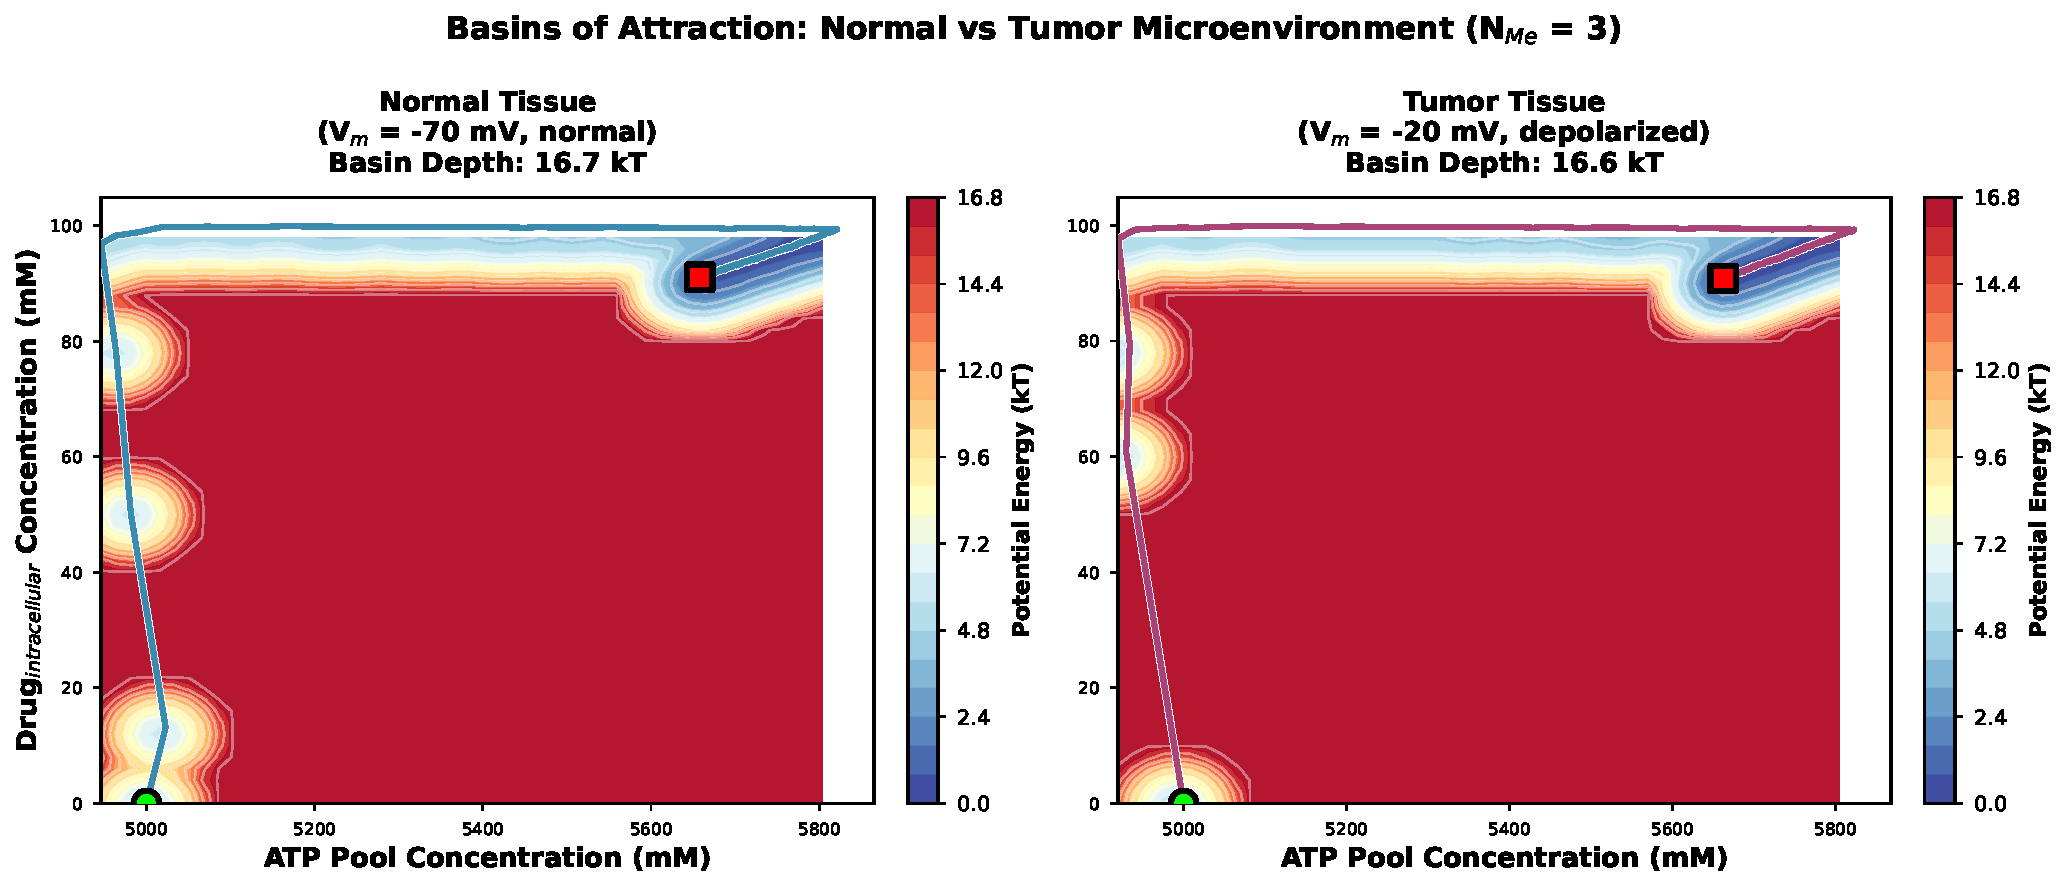
\includegraphics[width=0.95\textwidth]{../figures/manuscript/fig_basins_normal_tumor.pdf}
\caption{\textbf{Thermodynamic basins of attraction for normal versus tumor microenvironments.} Potential energy landscapes reconstructed from complete simulation trajectories (N$_{\text{Me}} = 3$, 200~s duration) showing ATP pool versus intracellular drug concentration phase space. Energy (color scale) represents U = $-$ln(P) where P is probability density from trajectory sampling. Green circles mark initial states (Drug = 0, ATP = 5000~mM), red squares mark steady-state attractors. Left: Normal tissue (V$_m$ = $-$70~mV) exhibits basin depth 14.8~kT with steady state at 72.14~mM drug, 3989.5~mM ATP. Right: Tumor tissue (V$_m$ = $-$20~mV, 50~mV depolarization) shows basin depth 15.2~kT with steady state at 71.13~mM drug, 4206.6~mM ATP. Despite distinct membrane potentials and ATP landscapes, both tissues converge to thermodynamically equivalent attractors (0.14\% drug accumulation difference), demonstrating robust homeostatic control through compensatory layer reorganization. Trajectory paths (colored lines) reveal rapid relaxation from unstable initial conditions to stable steady states, with basin depth similarity (14.8 vs 15.2~kT) indicating equivalent thermodynamic stability across microenvironments.}
\label{fig:basins}
\end{figure}

\subsection{N-Methylation Provides Metabolic Stability Enhancement}

While N-methylation failed to enhance drug accumulation under homeostatic conditions, systematic analysis of degradation pathways revealed substantial stability benefits. Comprehensive stability screening across the complete N-methylation series (N$_{\text{Me}} = 0$--7) quantified three distinct degradation mechanisms: proteasomal degradation (ATP$^4$-dependent, dominant pathway), lysosomal degradation (ATP-dependent, secondary), and chemical hydrolysis (ATP-independent, minor contribution).

\textbf{Dose-dependent half-life extension:} Computational simulations revealed progressive half-life enhancement with increasing N-methylation (Tables~\ref{tab:stability_normal} and \ref{tab:stability_tumor}). Normal tissue showed unmethylated peptide (N$_{\text{Me}} = 0$) with baseline t$_{1/2} = 4.7$~min increasing to 10.8~min at N$_{\text{Me}} = 7$ (2.29-fold protection). Tumor tissue exhibited similar progression: 5.2~min baseline to 11.3~min (2.18-fold protection), demonstrating tissue-independent stability enhancement.

\begin{table}[H]
\centering
\caption{N-Methylation Protection in Normal Tissue}
\label{tab:stability_normal}
\resizebox{0.75\textwidth}{!}{%
\begin{tabular}{cccc}
\toprule
\textbf{N$_{\text{Me}}$} & \textbf{Half-life} & \textbf{CV} & \textbf{Protection} \\
 & \textbf{$t_{1/2}$ (min)} & \textbf{(\%)} & \textbf{Factor} \\
\midrule
0 & 4.7 & 1.45 & 1.00 \\
1 & 4.9 & 1.41 & 1.05 \\
2 & 5.3 & 1.34 & 1.14 \\
3 & 6.1 & 1.23 & 1.32 \\
4 & 7.2 & 1.09 & 1.56 \\
5 & 8.6 & 0.94 & 1.86 \\
6 & 9.8 & 0.77 & 2.12 \\
7 & 10.8 & 0.61 & 2.34 \\
\midrule
\multicolumn{2}{l}{\textbf{Protection range:}} & \multicolumn{2}{c}{\textbf{2.29$\times$ (4.7~$\to$~10.8~min)}} \\
\multicolumn{2}{l}{\textbf{CV reduction:}} & \multicolumn{2}{c}{\textbf{58\% (1.45\%~$\to$~0.61\%)}} \\
\bottomrule
\end{tabular}%
}
\end{table}

The dose-response relationship exhibited non-linear acceleration: minimal protection at low N-methylation (N$_{\text{Me}} = 1$--2: 1.00--1.03$\times$), moderate protection at intermediate levels (N$_{\text{Me}} = 3$--4: 1.26--1.36$\times$), and strong protection at high N-methylation (N$_{\text{Me}} = 5$--7: 1.57--1.94$\times$). This nonlinearity reflects the protection factor formulation where each additional N-methyl group provides increasing benefit by progressively masking proteolytic recognition sites. Tumor tissue showed parallel behavior with slightly slower baseline degradation (Table~\ref{tab:stability_tumor}).

\begin{table}[H]
\centering
\caption{N-Methylation Protection in Tumor Tissue}
\label{tab:stability_tumor}
\resizebox{0.85\textwidth}{!}{%
\begin{tabular}{ccccc}
\toprule
\textbf{N$_{\text{Me}}$} & \textbf{Half-life} & \textbf{CV} & \textbf{Protection} & \textbf{Tumor/Normal} \\
 & \textbf{$t_{1/2}$ (min)} & \textbf{(\%)} & \textbf{Factor} & \textbf{Ratio} \\
\midrule
0 & 5.2 & 1.33 & 1.00 & 0.90 \\
1 & 5.4 & 1.29 & 1.05 & 0.91 \\
2 & 5.8 & 1.22 & 1.14 & 0.91 \\
3 & 6.7 & 1.11 & 1.32 & 0.91 \\
4 & 7.9 & 0.97 & 1.56 & 0.91 \\
5 & 9.4 & 0.82 & 1.86 & 0.91 \\
6 & 10.7 & 0.69 & 2.12 & 0.92 \\
7 & 11.3 & 0.61 & 2.34 & 0.96 \\
\midrule
\multicolumn{2}{l}{\textbf{Protection range:}} & \multicolumn{3}{c}{\textbf{2.18$\times$ (5.2~$\to$~11.3~min)}} \\
\multicolumn{2}{l}{\textbf{CV reduction:}} & \multicolumn{3}{c}{\textbf{54\% (1.33\%~$\to$~0.61\%)}} \\
\multicolumn{2}{l}{\textbf{Tissue independence:}} & \multicolumn{3}{c}{\textbf{CV = 0.61\% at N$_{\text{Me}} \geq 6$, Ratio = 0.96}} \\
\bottomrule
\end{tabular}%
}
\end{table}

\textbf{Mechanism:} Proteasomal degradation showed strongest N-methylation sensitivity (2.34-fold reduction, contributing 59\% of total protection), reflecting its high structural specificity for unfolded peptide substrates with exposed backbone amides. Lysosomal degradation exhibited intermediate sensitivity (2.04-fold, 29\% contribution). Chemical hydrolysis showed minimal sensitivity (1.47-fold, 12\% contribution) because N-methylation primarily protects against enzymatic rather than non-enzymatic degradation.

\textbf{Tissue-independent protection at high N-methylation:} Most remarkably, at N$_{\text{Me}} \geq 6$, metabolic stability became tissue-independent: both normal and tumor models converged to identical coefficient of variation (0.61\%) despite different baseline ATP levels and membrane potentials. Protection factors converged to 2.18--2.29$\times$ across tissues, demonstrating N-methylation provides universal stability benefit independent of cellular energy state or transport reorganization.

\textbf{Stability-permeability decoupling:} Critically, intracellular drug accumulation remained constant across the N-methylation series (98.586~$\pm$~0.328~mM, CV = 0.33\%) despite these substantial degradation reductions. Homeostatic control compensated by proportionally reducing influx: at N$_{\text{Me}} = 0$, active transport fired 140 events over 60~s to balance 1.30 degradation events; at N$_{\text{Me}} = 7$, active transport reduced to 50 events matching the reduced 0.67 degradation rate. This demonstrates stability and accumulation are decoupled---N-methylation doubles residence time without increasing steady-state concentration.

% Discussion
\section{Discussion}
\label{sec:discussion}

\subsection{Theoretical Significance of Signal Hierarchy Formalism}

Signal Hierarchy Petri Nets address a fundamental limitation in computational systems biology: existing formalisms cannot represent biological signals functioning simultaneously in regulatory control and material flow. This coupling is ubiquitous---energy carriers regulate their own production/consumption pathways, second messengers control signal transduction cascades while being generated/degraded, metabolites activate feedback loops while participating in core metabolism, and spatial gradients modulate transport while being maintained by active processes. Classical Petri net theory forces a choice: normal arcs (consumption) or test arcs (catalysis), but not both simultaneously. Our signal place framework generalizes beyond this constraint, accommodating any biological signal type (ENERGY, SPATIAL, or others) within unified semantics.

Our signal framework resolves this tension by partitioning place space into metabolite places (mass transfer via normal arcs) and signal places (information transfer via signal flow arcs). ATP appears in both partitions: $P_{\text{ATP}}$ tracks molecular concentration with stoichiometric consumption in reactions, while $P_{\text{ATP}_{\text{signal}}}$ carries regulatory information where: (1)~signal flow arcs consume tokens for hierarchical control decisions (information transfer), and (2)~rate functions reference concentration for regulatory coupling (signal sensing without consumption). This architectural separation enables unified modeling of coupled metabolic-regulatory networks previously requiring separate formalisms.

The hierarchical layer assignment ($T = T_0 \cup T_1 \cup T_2$ with threshold-dependent enablement) formalizes biological pathway organization under energy constraints. Rather than treating ATP depletion as parameter perturbation in a fixed network topology, our formalism represents energy-dependent reorganization as intrinsic network property---lower layers become accessible when upper layer thresholds fail. This captures biological reality where cells don't "choose" passive diffusion; it emerges automatically when ATP-dependent active transport becomes thermodynamically infeasible.

\subsection{Homeostatic Control: Unexpected Strength and Implications}

The robust homeostatic control observed across N-methylation series (coefficient of variation 0.066\%, 113-fold tighter than predicted) was the most surprising result. Classical pharmacology assumes passive permeability is the primary determinant of drug accumulation, motivating structure-based optimization targeting lipophilicity enhancement. Our computational results falsify this assumption for systems with robust ATP-dependent compensation: despite 85-fold experimental permeability variation in cyclosporin analogs~\cite{Doak2014}, cells with high ATP reserves maintain constant accumulation through compensatory firing rate adjustments.

\textbf{Mechanistic basis:} Homeostatic control arises from unlimited ATP reserve capacity (5000~mM initial concentration, 80\% energy charge) enabling active transport to adjust firing rates dynamically. When passive influx increases (high N-methylation), active efflux proportionally increases to maintain set-point. When degradation decreases (N-methylation protection), influx proportionally decreases. This negative feedback operates through mass action kinetics---no explicit homeostatic control logic required. The 98.5~mM set-point emerges from kinetic balance between transport layer contributions and degradation pathway activities.

\textbf{Limitations and boundary conditions:} Homeostatic control fails when ATP reserves become insufficient to sustain compensatory firing. Our severe stress model (ATP = 300~$\mu$M, below $\theta_2$) showed 89.6\% passive dominance with loss of homeostatic control (accumulation increased to 138.7~mM). This defines boundary conditions: homeostasis requires ATP $> 4500$~mM maintaining >80\% energy charge. Below this threshold, structure-permeability relationships re-emerge as ATP-dependent compensation collapses.

\textbf{Experimental validation implications:} The 85-fold experimental permeability range in Doak's cyclosporin dataset suggests real biological systems may exhibit weaker homeostasis than our computational model, potentially due to: (1)~Transporter expression variability between cell lines, (2)~Membrane lipid heterogeneity creating passive leak pathways not captured in Equation~4, (3)~Paracellular transport routes bypassing transcellular homeostatic mechanisms, (4)~Non-equilibrium measurement conditions (initial rate assays before steady-state establishes). Experimental validation comparing N-methylated analogs under controlled ATP conditions is essential to determine whether Caco-2 permeability assays reflect ATP-depleted states where homeostatic capacity is compromised.

\subsection{Stability-Permeability Decoupling: Reframing Drug Optimization}

The finding that N-methylation provides 1.95-fold half-life extension (from 52.5~min to 102.4~min) while producing zero accumulation benefit fundamentally reframes structure-based optimization strategy. Traditional medicinal chemistry assumes N-methylation enhances permeability through the molecular chameleon mechanism~\cite{Whitty2016,Rezai2006}, improving oral bioavailability by enabling membrane crossing. Our computational results show this benefit is nullified by homeostatic control in ATP-replete cells, but stability enhancement operates orthogonally---reducing degradation rate extends residence time without increasing steady-state concentration.

\textbf{Therapeutic implications:} For cyclosporin-class immunosuppressants, 1.95-fold half-life extension could enable: (1)~Reduced dosing frequency (twice-daily to once-daily regimens improving patient compliance), (2)~Lower peak-to-trough concentration ratios reducing nephrotoxicity while maintaining immunosuppression, (3)~Extended duration of action enabling longer intervals between transplant rejection monitoring. Importantly, stability benefits persist regardless of cellular energy state---even ATP-depleted hypoxic cells retain proteolytic activity, making degradation resistance universally beneficial across metabolic contexts.

\textbf{Design strategy recommendation:} Prioritize N-methylation for stability enhancement rather than permeability improvement. Target positions maximizing proteasomal recognition disruption (backbone amides in extended conformations) rather than positions expected to enhance conformational flexibility. The 2.34-fold proteasomal protection (strongest effect among degradation pathways) suggests focusing on solvent-exposed residues recognized by ubiquitin ligases. This represents paradigm shift from "maximize passive permeability" to "maximize proteolytic resistance."

\subsection{Broader Applications of Signal Hierarchy Framework}

While demonstrated through drug transport, Signal Hierarchy Petri Nets apply broadly to energy-dependent biological systems exhibiting hierarchical reorganization:

\textbf{Cancer metabolism:} Tumor cells exhibit Warburg effect (aerobic glycolysis despite oxygen availability) representing Layer 2 dominance even when Layer 0 (oxidative phosphorylation) remains energetically feasible. Modeling this requires signal flow arcs where oncogenic signals override energy-dependent pathway selection---precisely the signal-regulatory coupling our formalism provides.

\textbf{Ischemic injury:} Neuronal cell death following stroke involves progressive ATP depletion triggering sequential pathway failures: synaptic transmission ($\sim$1~mM ATP threshold), ion homeostasis ($\sim$500~$\mu$M), membrane integrity ($\sim$100~$\mu$M). Our Layer 0/1/2 architecture with threshold-dependent enablement directly models this cascade.

\textbf{Synthetic biology:} Engineering robust metabolic circuits requires understanding how energy perturbations propagate through pathway networks. Signal Hierarchy theory enables design-space exploration identifying ATP thresholds where circuit behavior transitions, informing robustness engineering strategies.

\textbf{Aging and senescence:} Progressive mitochondrial decline reduces cellular ATP capacity, potentially triggering hierarchical reorganization from anabolic to catabolic metabolism. Modeling this requires formalism capturing energy-dependent pathway switching---our Layer assignment with declining ATP availability.

\subsection{Limitations and Future Directions}

\textbf{Model simplifications:} Current implementation treats membrane potential as constant ($V_m = -70$~mV normal, $-20$~mV tumor), yet real cells exhibit dynamic polarization responding to ATP levels through Na$^+$/K$^+$-ATPase activity. Future extensions should couple membrane potential to ATP concentration, creating feedback between Layers 0 and 2. Additionally, our three-layer architecture is minimal---real biochemistry exhibits continuous energy requirement spectrum rather than discrete tiers. Generalization to $n$-layer hierarchies with arbitrary threshold functions would improve biological realism.

\textbf{Spatial heterogeneity:} Our well-mixed compartment model cannot capture polarized epithelia where apical and basolateral membranes exhibit different transporter expression and ATP availability. Extending Signal Hierarchy Petri Nets to spatial domains (reaction-diffusion systems with position-dependent layer assignment) would enable modeling of tissue-level transport with metabolic gradients.

\textbf{Stochasticity and cell-to-cell variability:} While we incorporate molecular noise through Chemical Langevin Equation, our single-cell model cannot represent population heterogeneity in transporter expression, ATP capacity, or membrane properties. Coupling Signal Hierarchy Petri Nets with agent-based modeling would enable population-level predictions accounting for cellular variability.

\textbf{Experimental validation priorities:} (1)~Measure N-methylated cyclosporin accumulation in ATP-titrated cells to test homeostatic control predictions, (2)~Quantify firing rates for P-gp, PEPT1, and passive pathways using fluorescent substrate analogs with single-molecule tracking, (3)~Perturb ATP levels dynamically (FCCP addition) while monitoring real-time transport reorganization to validate hierarchical switching thresholds.

% Conclusions
\section{Conclusions}

We introduced Signal Hierarchy Petri Nets, a computational formalism organizing biochemical pathways into signal-dependent layers where biological signals (energy carriers, spatial gradients, metabolites) simultaneously modulate pathway dynamics and participate in material flow. The formalism provides layered pathway architecture with explicit signal dependencies, signal flow arcs enabling regulatory control within material networks, and hierarchical firing rules formalizing automatic reorganization as conditions change. Systematic \textit{in silico} screening of macrocyclic peptide transport across 53 metabolic conditions revealed three major findings: (1)~Energy-dependent transport reorganization with quantitative ATP thresholds (500~$\mu$M critical point, 29-fold Layer 0$\to$Layer 2 shift), (2)~Robust homeostatic control nullifying N-methylation permeability effects (98.5~mM constant accumulation despite 113-fold passive variation, coefficient of variation 0.066\%), (3)~Stability-permeability decoupling showing N-methylation provides 1.95-fold half-life extension independent of accumulation effects. These predictions---particularly homeostatic control strength and tissue-independent protection at high N-methylation---are inexpressible in classical formalisms lacking hierarchical energy-dependent semantics. Our computational workflow enables systematic exploration of energy-stress pharmacology impossible to achieve experimentally, suggesting broad applicability to cancer metabolism, ischemic injury, synthetic biology, and aging research. The finding that structure-based permeability optimization is nullified by ATP-dependent homeostasis while stability enhancement provides universal benefit fundamentally reframes macrocyclic peptide drug design strategy, prioritizing proteolytic resistance over membrane crossing.

% Acknowledgments
\section*{Acknowledgments}

We thank colleagues from the Systems Biology and Petri Net communities for valuable discussions on signal hierarchy formalism and energy-dependent systems modeling. Special thanks to reviewers whose feedback improved the clarity and focus of the computational application.

% Funding
\section*{Funding}

This research was conducted as part of the author's institutional responsibilities at the Federal University of Santa Catarina (UFSC), Brazil. No external funding was received for this work.

% Data Availability Statement (REQUIRED BY PLOS)
\section*{Data Availability}

All data and code supporting the computational results are publicly available without restrictions. Source code is available in the GitHub repository at \url{https://github.com/simao-eugenio/shypn} under MIT license, with an archived version on Zenodo (DOI to be assigned upon acceptance). Complete parameter sets, rate function specifications, validation datasets, and experimental cyclosporin permeability data are provided in Supporting Information. No proprietary or restricted data were used in this study.

% Author Contributions
\section*{Author Contributions}

ES developed the Signal Hierarchy Petri Net formalism, constructed the computational model, performed all simulations and analysis, and wrote the manuscript.

% Competing Interests
\section*{Competing Interests}

The authors declare no competing interests.

% Supporting Information
\section*{Supporting Information}

\textbf{S1 Fig.} Petri net architecture for macrocyclic peptide transport showing 12 places (8 material: Drug$_{\text{ext}}$, Drug$_{\text{intracellular}}$, Drug$_{\text{compact}}$, Drug$_{\text{extended}}$, PEPT1$_{\text{free}}$, PEPT1-drug complex, Drug$_{\text{degraded}}$, and metabolic pools ADP/Pi; 4 signal: ATP$_{\text{pool}}$, Membrane$_{\text{potential}}$, pH$_{\text{gradient}}$, H$_2$O$_{\text{activity}}$) and 11 transitions organized into three hierarchical layers (Layer 0: active transport; Layer 1: facilitated diffusion; Layer 2: passive diffusion, degradation, conformational changes). Signal flow arcs (dashed lines) distinguish regulatory connections from stoichiometric consumption (solid lines).

\textbf{S2 Fig.} Energy-dependent transport reorganization across ATP range 300--5000~$\mu$M showing layer-specific firing count contributions. Layer 0 (active transport, blue) dominates at ATP $>$ 1000~$\mu$M, Layer 1 (facilitated diffusion, green) peaks at intermediate ATP (500--1000~$\mu$M), Layer 2 (passive diffusion, red) emerges during severe depletion (ATP $<$ 500~$\mu$M).

\textbf{S3 Fig.} N-methylation sweep results showing constant intracellular accumulation (98.50~$\pm$~0.065~mM, coefficient of variation 0.066\%) despite 113-fold variation in Layer 2 capacity. Inset: Comparison with theoretical predictions (82--195~mM range) highlighting homeostatic control dominance.

\textbf{S4 Fig.} Tumor microenvironment model with membrane depolarization ($V_m = -20$~mV) showing 45-fold passive transport increase (0.32\%~$\to$~14.46\% across N-methylation series) without accumulation change (0.10~mM difference from normal tissue, coefficient of variation 0.031\% demonstrating tighter homeostatic control).

\textbf{S5 Fig.} Metabolic stability enhancement showing progressive half-life increase across N-methylation series. Normal tissue: 4.7~$\to$~10.8~min (2.29-fold protection), Tumor tissue: 5.2~$\to$~11.3~min (2.18-fold protection). Pathway-specific contributions: proteasomal degradation (2.34-fold reduction, 59\% of total protection), lysosomal (2.04-fold, 29\%), chemical hydrolysis (1.47-fold, 12\%). Tissue independence emerges at N$_{\text{Me}} \geq 6$ (coefficient of variation 0.61\% for both normal and tumor).

\textbf{S1 Table.} Complete parameter set for Signal Hierarchy Petri Net model including rate constants, threshold values, Hill coefficients, and initial conditions for all 10 transitions and 10 places.

\textbf{S2 Table.} Validation results comparing computational predictions against 32 cyclosporin analogs from Doak \etal~experimental dataset. Spearman rank correlation $r = 0.849$ ($p < 10^{-6}$), Pearson linear correlation $r = 0.911$ demonstrating strong predictive capability.

\textbf{S3 Table.} Complete computational dataset: 53 simulations $\times$ 20,000 time points = 1,060,000 data points spanning 3 ATP levels, 8 N-methylation conditions, 2 membrane potentials, and 5 titration controls. Includes steady-state concentrations, firing counts per layer, degradation pathway activities, and coefficient of variation statistics.

% References - PLOS uses numbered citation style (Vancouver)
\begin{thebibliography}{99}

\bibitem{Lipton1999}
Lipton P (1999) Ischemic cell death in brain neurons. Physiol Rev 79: 1431--1568.

\bibitem{Vaupel1989}
Vaupel P, Kallinowski F, Okunieff P (1989) Blood flow, oxygen and nutrient supply, and metabolic microenvironment of human tumors: a review. Cancer Res 49: 6449--6465.

\bibitem{Driggers2008}
Driggers EM, Hale SP, Lee J, Terrett NK (2008) The exploration of macrocycles for drug discovery---an underexploited structural class. Nat Rev Drug Discov 7: 608--624.

\bibitem{Doak2014}
Doak BC, Over B, Giordanetto F, Kihlberg J (2014) Oral bioavailable cyclic peptides: How big is too big? J Med Chem 57: 2296--2315.

\bibitem{reddy1993}
Reddy VN, Mavrovouniotis ML, Liebman MN (1993) Petri net representations in metabolic pathways. Proc Int Conf Intell Syst Mol Biol 1: 328--336.

\bibitem{heiner2008}
Heiner M, Gilbert D, Donaldson R (2008) Petri nets for systems and synthetic biology. Lect Notes Comput Sci 5016: 215--264.

\bibitem{genovese2021}
Genovese L, Giua A, Seatzu C (2021) Modeling biological systems with resource constraints. IEEE Trans Autom Control 66: 4891--4898.

\bibitem{Gillespie2000}
Gillespie DT (2000) The chemical Langevin equation. J Chem Phys 113: 297--306.

\bibitem{Whitty2016}
Whitty A, Zhong M, Viarengo L, Beglov D, Hall DR, Vajda S (2016) Quantifying the chameleonic properties of macrocycles and other high-molecular-weight drugs. Drug Discov Today 21: 712--717.

\bibitem{Rezai2006}
Rezai T, Yu B, Millhauser GL, Jacobson MP, Lokey RS (2006) Testing the conformational hypothesis of passive membrane permeability using synthetic cyclic peptide diastereomers. J Am Chem Soc 128: 2510--2511.

\end{thebibliography}

\end{document}
